\documentclass[10pt]{article}
\usepackage[margin=1.7cm]{geometry}
\usepackage{libertine}
\usepackage{amsmath}
\usepackage{xcolor}
\usepackage{pgfplots}
\pgfplotsset{compat=1.18}
\pagestyle{empty}
\setlength{\parindent}{0pt}
\setlength{\parskip}{0.5em}

\definecolor{accent}{HTML}{8A3A5C}
\definecolor{spike}{HTML}{2E5C8A}

\newcommand{\heading}[1]{{\bfseries\color{accent} #1}}

\begin{document}

{\LARGE\bfseries\color{accent} Computational Neuroscience Notes}\\[0.1em]
{\large Lecture 9: the leaky integrate-and-fire neuron model}

\vspace{0.5em}
\heading{1. Membrane dynamics}

The leaky integrate-and-fire (LIF) model treats a neuron's membrane as an
RC circuit driven by an input current $I(t)$. The subthreshold membrane
potential $V(t)$ obeys
\[
  \tau_m \frac{dV}{dt} = -\big(V(t) - V_{\text{rest}}\big) + R\, I(t),
\]
where $\tau_m = R C$ is the membrane time constant, $V_{\text{rest}}$ is the
resting potential, and $R$ is the membrane resistance. Between spikes this
is a simple linear ODE: with constant input the membrane charges toward the
steady state $V_{\text{rest}} + R I$ with time constant $\tau_m$.

\heading{2. The threshold-and-reset rule}

The model becomes a spiking neuron by adding a nonlinear reset. Whenever
$V(t)$ reaches the threshold $V_{\text{th}}$,
\[
  V(t) \ge V_{\text{th}} \quad\Longrightarrow\quad
  \text{emit a spike, then set } V(t^+) = V_{\text{reset}},
\]
after which the subthreshold dynamics resume. This single rule, linear
charging plus an instantaneous reset, is enough to reproduce a wide range of
firing patterns seen in cortical recordings, provided $\tau_m$, $V_{\text{th}}$,
and the input statistics are chosen to match the cell being modeled.

\heading{3. Firing rate under constant drive}

For a constant suprathreshold current the inter-spike interval has a closed
form, giving the steady-state firing rate
\[
  f = \left[ \tau_m \ln\!\left( \frac{R I - (V_{\text{reset}} - V_{\text{rest}})}
  {R I - (V_{\text{th}} - V_{\text{rest}})} \right) \right]^{-1}.
\]
Increasing $I$ shortens each charging phase and raises $f$ smoothly, with no
sharp onset, in contrast to neurons that show a hard rheobase threshold.

\heading{4. Simulated membrane potential trace}

The trace below simulates Euler integration of the LIF equation with
$\tau_m = 10$ ms, $V_{\text{rest}} = -65$ mV, $V_{\text{th}} = -50$ mV, and
$V_{\text{reset}} = -70$ mV under constant input. Each vertical line marks a
spike, after which the potential resets and begins charging again.

\begin{center}
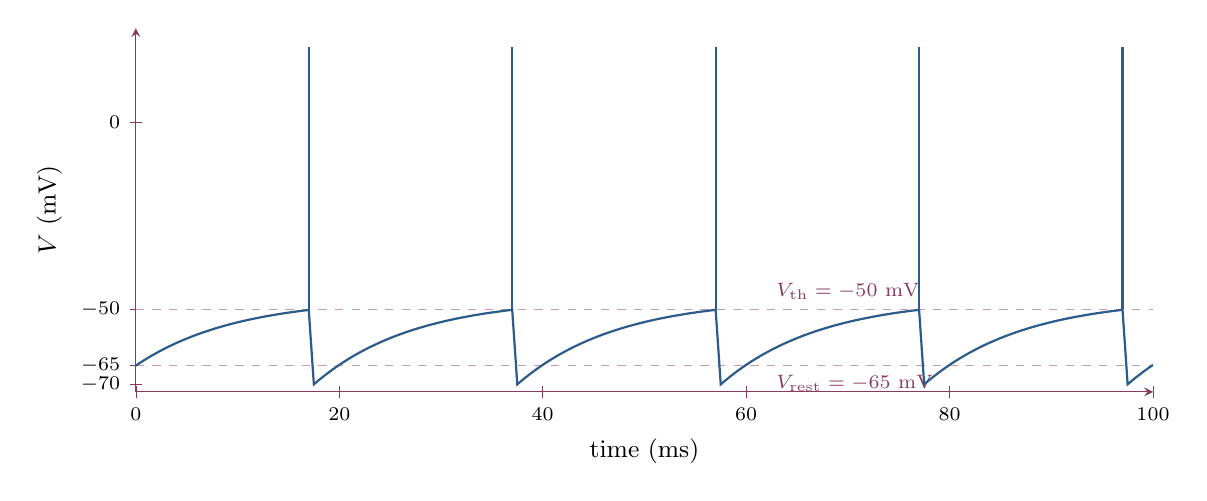
\begin{tikzpicture}
\begin{axis}[
    width=14.5cm, height=6.2cm,
    xlabel={time (ms)}, ylabel={$V$ (mV)},
    xmin=0, xmax=100, ymin=-72, ymax=25,
    axis lines=left,
    xtick={0,20,...,100}, ytick={-70,-65,-50,0},
    ticklabel style={font=\scriptsize},
    label style={font=\small},
    axis line style={accent}, tick style={accent},
    ]
  \draw[accent!50, dashed] (axis cs:0,-50) -- (axis cs:100,-50);
  \draw[accent!50, dashed] (axis cs:0,-65) -- (axis cs:100,-65);
  \node[accent, font=\scriptsize, anchor=south west] at (axis cs:62,-50) {$V_{\text{th}} = -50$~mV};
  \node[accent, font=\scriptsize, anchor=north west] at (axis cs:62,-65) {$V_{\text{rest}} = -65$~mV};

  \addplot[spike, thick] coordinates {
    (0.0,-65.0) (0.5,-64.1) (1.0,-63.24) (1.5,-62.43) (2.0,-61.66) (2.5,-60.93) (3.0,-60.23) (3.5,-59.57) (4.0,-58.94) (4.5,-58.34) (5.0,-57.78) (5.5,-57.24) (6.0,-56.73) (6.5,-56.24) (7.0,-55.78) (7.5,-55.34) (8.0,-54.92) (8.5,-54.53) (9.0,-54.15) (9.5,-53.79) (10.0,-53.45) (10.5,-53.13) (11.0,-52.82) (11.5,-52.53) (12.0,-52.26) (12.5,-51.99) (13.0,-51.74) (13.5,-51.51) (14.0,-51.28) (14.5,-51.07) (15.0,-50.86) (15.5,-50.67) (16.0,-50.49) (16.5,-50.31) (17.0,-50.15) (17.5,-70.0) (18.0,-68.85) (18.5,-67.76) (19.0,-66.72) (19.5,-65.73) (20.0,-64.8) (20.5,-63.91) (21.0,-63.06) (21.5,-62.26) (22.0,-61.5) (22.5,-60.77) (23.0,-60.08) (23.5,-59.43) (24.0,-58.81) (24.5,-58.22) (25.0,-57.66) (25.5,-57.12) (26.0,-56.62) (26.5,-56.14) (27.0,-55.68) (27.5,-55.25) (28.0,-54.83) (28.5,-54.44) (29.0,-54.07) (29.5,-53.72) (30.0,-53.38) (30.5,-53.06) (31.0,-52.76) (31.5,-52.47) (32.0,-52.2) (32.5,-51.94) (33.0,-51.69) (33.5,-51.46) (34.0,-51.23) (34.5,-51.02) (35.0,-50.82) (35.5,-50.63) (36.0,-50.45) (36.5,-50.28) (37.0,-50.11) (37.5,-70.0) (38.0,-68.85) (38.5,-67.76) (39.0,-66.72) (39.5,-65.73) (40.0,-64.8) (40.5,-63.91) (41.0,-63.06) (41.5,-62.26) (42.0,-61.5) (42.5,-60.77) (43.0,-60.08) (43.5,-59.43) (44.0,-58.81) (44.5,-58.22) (45.0,-57.66) (45.5,-57.12) (46.0,-56.62) (46.5,-56.14) (47.0,-55.68) (47.5,-55.25) (48.0,-54.83) (48.5,-54.44) (49.0,-54.07) (49.5,-53.72) (50.0,-53.38) (50.5,-53.06) (51.0,-52.76) (51.5,-52.47) (52.0,-52.2) (52.5,-51.94) (53.0,-51.69) (53.5,-51.46) (54.0,-51.23) (54.5,-51.02) (55.0,-50.82) (55.5,-50.63) (56.0,-50.45) (56.5,-50.28) (57.0,-50.11) (57.5,-70.0) (58.0,-68.85) (58.5,-67.76) (59.0,-66.72) (59.5,-65.73) (60.0,-64.8) (60.5,-63.91) (61.0,-63.06) (61.5,-62.26) (62.0,-61.5) (62.5,-60.77) (63.0,-60.08) (63.5,-59.43) (64.0,-58.81) (64.5,-58.22) (65.0,-57.66) (65.5,-57.12) (66.0,-56.62) (66.5,-56.14) (67.0,-55.68) (67.5,-55.25) (68.0,-54.83) (68.5,-54.44) (69.0,-54.07) (69.5,-53.72) (70.0,-53.38) (70.5,-53.06) (71.0,-52.76) (71.5,-52.47) (72.0,-52.2) (72.5,-51.94) (73.0,-51.69) (73.5,-51.46) (74.0,-51.23) (74.5,-51.02) (75.0,-50.82) (75.5,-50.63) (76.0,-50.45) (76.5,-50.28) (77.0,-50.11) (77.5,-70.0) (78.0,-68.85) (78.5,-67.76) (79.0,-66.72) (79.5,-65.73) (80.0,-64.8) (80.5,-63.91) (81.0,-63.06) (81.5,-62.26) (82.0,-61.5) (82.5,-60.77) (83.0,-60.08) (83.5,-59.43) (84.0,-58.81) (84.5,-58.22) (85.0,-57.66) (85.5,-57.12) (86.0,-56.62) (86.5,-56.14) (87.0,-55.68) (87.5,-55.25) (88.0,-54.83) (88.5,-54.44) (89.0,-54.07) (89.5,-53.72) (90.0,-53.38) (90.5,-53.06) (91.0,-52.76) (91.5,-52.47) (92.0,-52.2) (92.5,-51.94) (93.0,-51.69) (93.5,-51.46) (94.0,-51.23) (94.5,-51.02) (95.0,-50.82) (95.5,-50.63) (96.0,-50.45) (96.5,-50.28) (97.0,-50.11) (97.5,-70.0) (98.0,-68.85) (98.5,-67.76) (99.0,-66.72) (99.5,-65.73) (100.0,-64.8)
  };

  \addplot[spike, thick] coordinates {(17.0,-50) (17.0,20)};
  \addplot[spike, thick] coordinates {(37.0,-50) (37.0,20)};
  \addplot[spike, thick] coordinates {(57.0,-50) (57.0,20)};
  \addplot[spike, thick] coordinates {(77.0,-50) (77.0,20)};
  \addplot[spike, thick] coordinates {(97.0,-50) (97.0,20)};
\end{axis}
\end{tikzpicture}
\end{center}

\heading{5. Reading the trace}

Between spikes the potential climbs monotonically toward the driven steady
state, slowing as it approaches $V_{\text{th}}$ because the driving term
$R I - (V - V_{\text{rest}})$ shrinks. The five spikes shown are evenly
spaced because the input current is constant, an inter-spike interval of
20 ms corresponds to a firing rate of 50 Hz for this parameter set.

\end{document}
